%%
% Please see https://bitbucket.org/rivanvx/beamer/wiki/Home for obtaining beamer.
%%
\documentclass{beamer}
\usepackage{natbib}
\usepackage{graphicx}
\usetheme{Singapore}
\usepackage{subfig}
\usepackage{dcolumn}
\usepackage{hyperref}
\title[] %optional
{Using LDA to Identify Knowledge Capital Risks in Annual Reports}

\author[Pedro Vallocci] % (optional)
{Pedro H. Braz Vallocci\inst{1}}

\institute[UCSC] % (optional)
{
  \inst{1}%
  University of California, Santa Cruz
 }

\newcommand{\ffo}{dicfullmc10thr10defnob5noa0_8_4t}
\newcommand{\ffoiii}{dicfullmc10thr10defnob5noa0_8_3t}
\newcommand{\ffovi}{dicfullmc10thr10defnob5noa0_8_6t}

\newcommand{\insertfigurenoffo}[3]{
\begin{figure}[h!]
  \centering
  \includegraphics[width=#3\textwidth]{#1}
  \caption{#2}
  \label{fig:#1}
\end{figure}
}

\newcommand{\insertfigure}[2]{
\begin{figure}[h!]
  \centering
  \includegraphics[width=0.6\textwidth]{\ffo/#1}
  \centering
  \captionsetup{font=scriptsize}
  \caption{#2}
  \label{fig:#1}
\end{figure}
}

\newcommand{\insertfigureiii}[2]{
\begin{figure}[h!]
  \centering
  \includegraphics[width=0.6\textwidth]{\ffoiii/#1}
  \centering
  \captionsetup{font=scriptsize}
  \caption{#2}
  \label{fig:#1}
\end{figure}
}

\newcommand{\insertfigurevi}[2]{
\begin{figure}[h!]
  \centering
  \includegraphics[width=0.6\textwidth]{\ffovi/#1}
  \centering
  \captionsetup{font=scriptsize}
  \caption{#2}
  \label{fig:#1}
\end{figure}
}


\begin{document}
\frame{\titlepage}

\begin{frame}
\frametitle{Outline}
\tableofcontents
\end{frame}

\section{Introduction}
\begin{frame}
\frametitle{Motivation}
\begin{itemize}	
\item \textit{Knowledge capital} represents a firm's cumulative investment in research and development (R\&D) and constitutes a significant portion (38 to 47\%) of its overall value (\cite{Belo2019-iz}).
\item Knowledge capital differs from physical capital in terms of its risk profile:
\begin{itemize}
\item It incurs higher adjustment costs (Belo et al., 2019), experiences greater depreciation (Li et al., 2020), and is subject to factors such as obsolescence and patent breaks.
\item The outcomes of R\&D investments are uncertain, leading to increased volatility in cash flows (Andrei et al., 2019).
\end{itemize}



\end{itemize}
\end{frame}


\begin{frame}
\frametitle{Research question}
  \begin{itemize}
  \item Existing measures are insufficient for identifying knowledge-heavy firms:
\begin{itemize}
\item Inconsistent standards for R\&D reporting across industries and firms, with some firms not disclosing R\&D expenditure in their annual reports.
\item Intangible asset measures done through indirect measures (SG\&A) encompass non-knowledge-related components of organizational capital.
\item Patents only capture the final outcomes of R\&D investment, neglecting the internal learning process within firms.
\end{itemize}
\item Research questions:
\begin{itemize}
\item Can we identify knowledge-heavy firms by performing text analysis on the risk factors reported in their annual reports?
\item If so, do agents price in different risks for knowledge-heavy firms?
\item More generally, can topic modeling the firms' self-declared risk factor provide a sensible categorization of firms by risk?
\end{itemize}
\end{itemize}
\end{frame}


\begin{frame}
\frametitle{Approach}
\begin{itemize}
\item I employ Latent Dirichlet Allocation (LDA), a topic modeling technique, on a corpus of 121,839 firm annual reports (2006-2022), to identify latent topics.
\item By matching firms based on their CIK and PERMNO, I link the annual reports to daily stock data (aggregated weekly), Compustat data, and measures of firms' knowledge capital, accumulated patent value, and industry skill from existing literature.
\item I observe a positive association between higher intensities of a specific topic (e.g., "topic kk") and the aforementioned measures. Moreover, firms in the upper quartile of "topic\_kk" have outperformed their peers in terms of returns since 2006.
\end{itemize}

\end{frame}

\section{Data}

\begin{frame}
\frametitle{Latent Dirichlet Allocation (LDA)}
\begin{itemize}
\small
\item LDA is a generative statistical model widely used for topic modelling in natural language processing (NLP).
\item It operates under the assumption that each document in a corpus is a mixture of a number of latent topics $k \in \{1, ..., K\}$, with weights $\omega_{i1}, ..., \omega_{iK}$. Each topic is assigned a word probability vector $\mathbf{\theta}_k$. 
\item Therefore, if $X_i$ is the vector of word counts with length $n_i$, 
\begin{equation}
X_i \sim \operatorname{Multinomial}\left(n_i, \omega_{i 1} \theta_1+\cdots+\omega_{i K} \theta_K\right)
\end{equation}
\item The output of LDA is a list of topics, each represented as a collection of words, and a weight distribution across these topics for each document.
\item LDA is an unsupervised learning method, meaning that it learns and infers from the data without any predefined labels.
\end{itemize}
\end{frame}

\begin{frame}
  \frametitle{An example of 10-K}
\insertfigurenoffo{apples_1a}{A slice of Apple's 10-K (Item 1A, Risk Factors)}{0.8}
\end{frame}

\begin{frame}
\frametitle{10-K data processing steps}
\begin{figure}[h!]
  \centering
  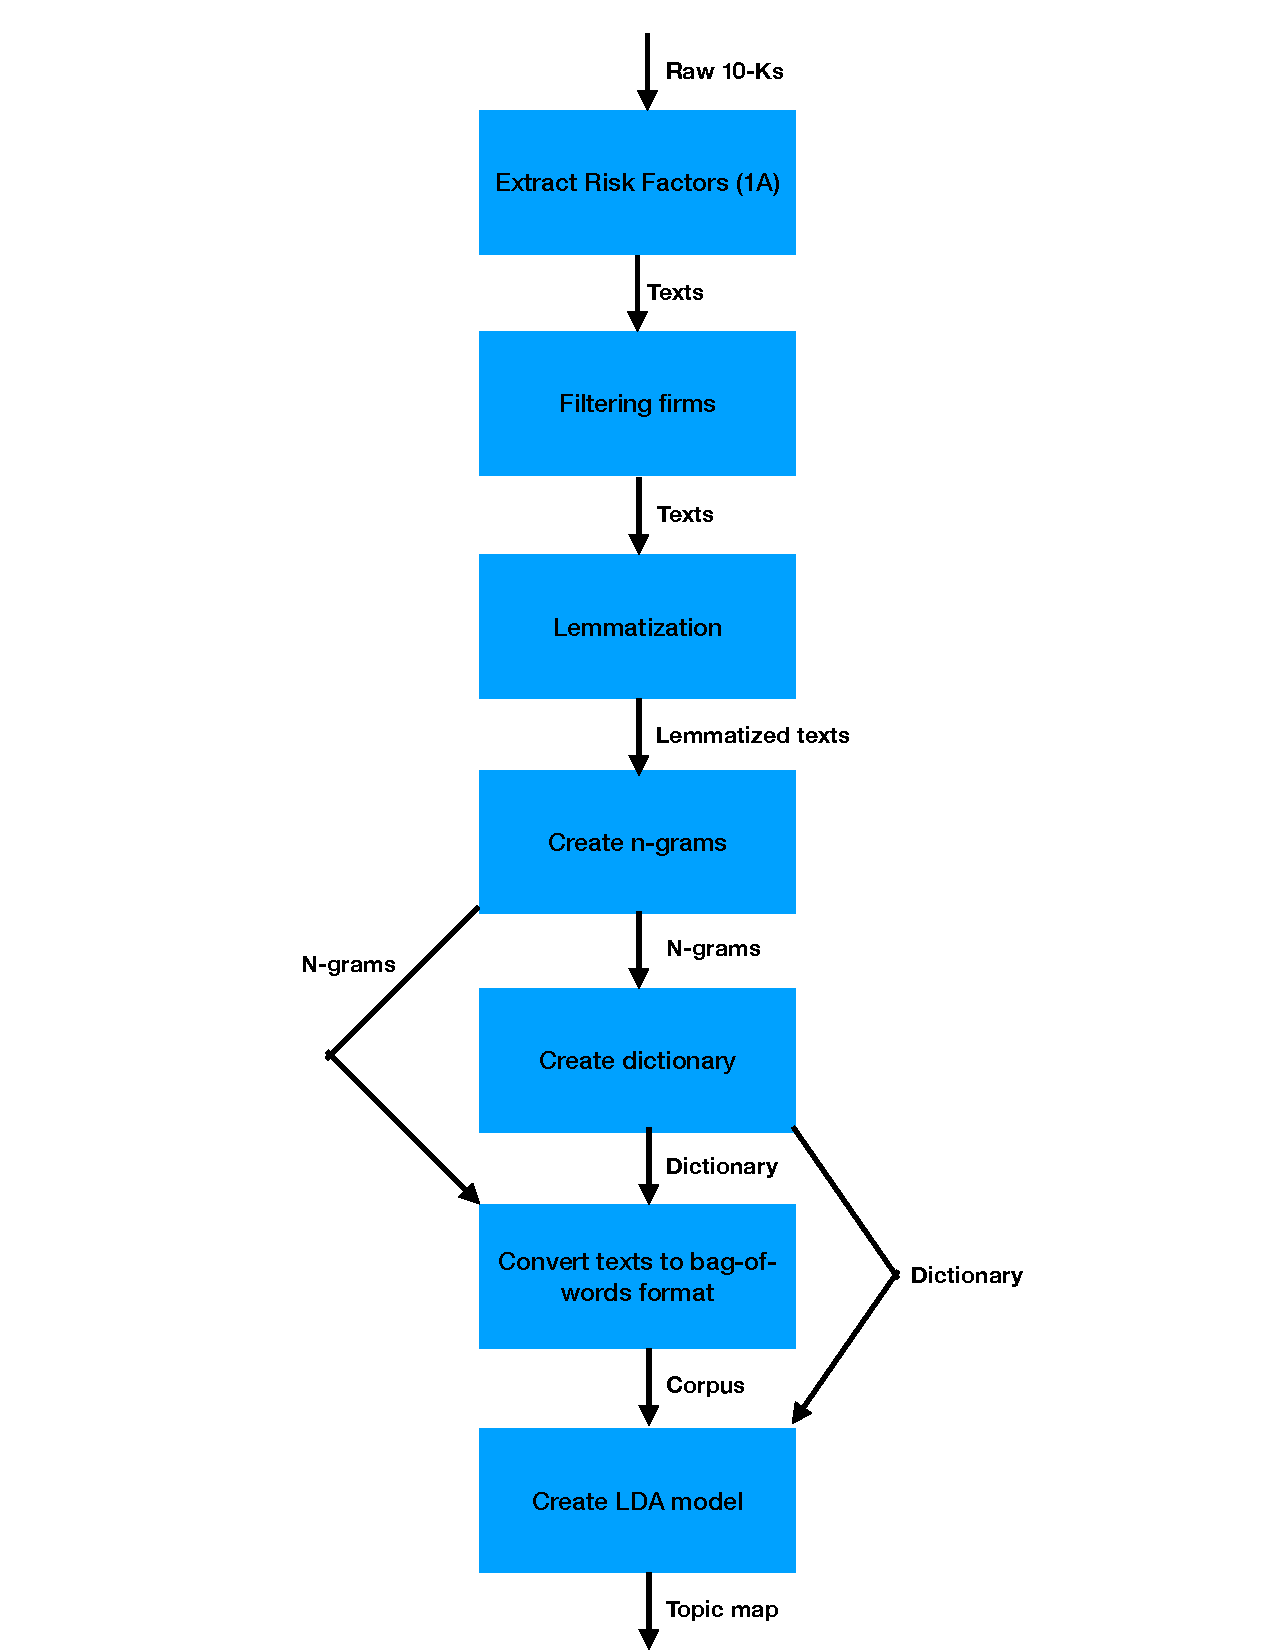
\includegraphics[width=0.5\textwidth]{data_steps.pdf}
  \caption{Data processing steps}
  \label{data_steps}
\end{figure}
\end{frame}

\begin{frame}
\frametitle{Downloading 10-Ks and extracting risk factors}
\begin{itemize}
\item Downloaded from the SEC website 121,839 firm 10-Ks, filed from 2006 to 2022, resulting in approximately 1.6 TB of data. Each 10-K is stored as raw HTML code
\item Extracted the Item 1A (Risk Factors) section from the tree-like structure of each 10-K.
\item Parsed the text from the Item 1A section using \texttt{BeautifulSoup}; removed punctuation and numbers.
\end{itemize}
\end{frame}


\begin{frame}
\frametitle{Filtering firms (1)}
\begin{itemize}
\item Only ordinary common shares, traded at NYSE, AMEX, or NASDAQ, are kept (\cite{Stambaugh2016-eb}, \cite{Golubov2019-ku}):
\begin{itemize}
  \item I also consider only firms whose stocks were being traded at a minimum price of \$5 in 2016 dollars (\cite{Stambaugh2016-eb})
\end{itemize}
\end{itemize}
\end{frame}



\begin{frame}
\frametitle{Filtering firms (2)}
\begin{itemize}
\item Reporting risk factors is mandatory for most firms, but there are exceptions for asset-backed issuers and smaller reporting companies.
\item Asset-backed issuers are defined as issuers whose reporting obligation arises from the registration of an offering of asset-backed securities under the Securities Act or the registration of a class of asset-backed securities.
\item Firms that are not required to disclose risk factors may leave Item 1A empty or write a placeholder text indicating that they are not required to disclose risk factors due to their nature.
\item This leads to a high frequency of 10-K filings with a significantly low number of words, as shown in Figure \ref{fig:cdf}. In the subsequent stages, 1A texts with an insufficient word count (less than 200 words) are discarded.

\end{itemize}
\end{frame}

\begin{frame}
\frametitle{Filtering firms (3)}
\begin{figure}
  \centering
  \subfloat[Full picture]{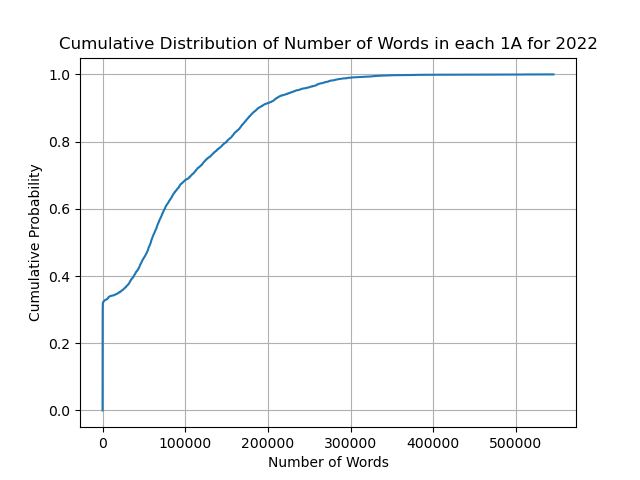
\includegraphics[width=0.45\textwidth]{cdf_words}\label{fig:cdf_words}}
  \hfill
  \subfloat[Detail]{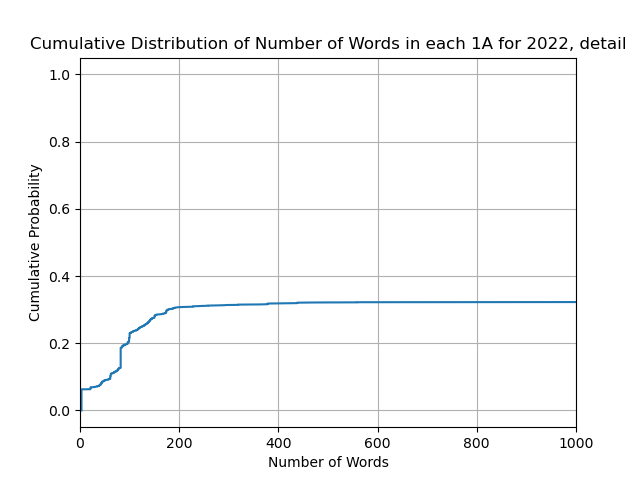
\includegraphics[width=0.45\textwidth]{cdf_words_zoom}\label{fig:cdf_words_zoom}}
  \caption{Word count cumulative distribution function, for all 10-Ks filed in 2022}
  \label{fig:cdf}
\end{figure}
\end{frame}

\begin{frame}
\frametitle{Filtering firms (4)}
\scriptsize

\begin{table}[!htbp] \centering 

  \label{tab:file_counts} 
\begin{tabular}{@{\extracolsep{5pt}} D{.}{.}{-3} D{.}{.}{-3} D{.}{.}{-3} } 
\\[-1.8ex]\hline 
\hline \\[-1.8ex] 
\multicolumn{1}{c}{Year} & \multicolumn{1}{c}{Total\_1As} & \multicolumn{1}{c}{Filtered} \\ 
\hline \\[-1.8ex] 
\multicolumn{1}{c}{2006} & \multicolumn{1}{c}{5685} & \multicolumn{1}{c}{2466} \\ 
\multicolumn{1}{c}{2007} & \multicolumn{1}{c}{6445} & \multicolumn{1}{c}{2714} \\ 
\multicolumn{1}{c}{2008} & \multicolumn{1}{c}{6931} & \multicolumn{1}{c}{2305} \\ 
\multicolumn{1}{c}{2009} & \multicolumn{1}{c}{8244} & \multicolumn{1}{c}{2190} \\ 
\multicolumn{1}{c}{2010} & \multicolumn{1}{c}{8122} & \multicolumn{1}{c}{2290} \\ 
\multicolumn{1}{c}{2011} & \multicolumn{1}{c}{8019} & \multicolumn{1}{c}{2356} \\ 
\multicolumn{1}{c}{2012} & \multicolumn{1}{c}{7797} & \multicolumn{1}{c}{2316} \\ 
\multicolumn{1}{c}{2013} & \multicolumn{1}{c}{7560} & \multicolumn{1}{c}{2401} \\ 
\multicolumn{1}{c}{2014} & \multicolumn{1}{c}{7560} & \multicolumn{1}{c}{2518} \\ 
\multicolumn{1}{c}{2015} & \multicolumn{1}{c}{7531} & \multicolumn{1}{c}{2528} \\ 
\multicolumn{1}{c}{2016} & \multicolumn{1}{c}{7196} & \multicolumn{1}{c}{2431} \\ 
\multicolumn{1}{c}{2017} & \multicolumn{1}{c}{6896} & \multicolumn{1}{c}{2394} \\ 
\multicolumn{1}{c}{2018} & \multicolumn{1}{c}{6804} & \multicolumn{1}{c}{2418} \\ 
\multicolumn{1}{c}{2019} & \multicolumn{1}{c}{6683} & \multicolumn{1}{c}{2404} \\ 
\multicolumn{1}{c}{2020} & \multicolumn{1}{c}{6531} & \multicolumn{1}{c}{2332} \\ 
\multicolumn{1}{c}{2021} & \multicolumn{1}{c}{6936} & \multicolumn{1}{c}{2308} \\ 
\multicolumn{1}{c}{2022} & \multicolumn{1}{c}{6899} & \multicolumn{1}{c}{1885} \\ 
\hline \\[-1.8ex] 
\end{tabular} 
\caption{The left column shows the count of all 10-Ks retrieved for a given year. The right column counts all the 10-Ks that obey to the following filtering criteria: 1) Ordinary common shares; 2) Membership to NYSE, AMEX, and NASDAQ; 3) Price above \$ 5 in 2006 dollars; 4) Meaningful 10-K contents ($>$ 200 words)} 
\end{table} 


\end{frame}


\begin{frame}
\frametitle{The Process of Lemmatization}
\begin{itemize}
\item Lemmatization is the technique of converting words to their base or root form, effectively eliminating any suffixes and inflections. This ensures semantic consistency across different forms of a word.
\begin{itemize}
  \item For instance, words like "take", "took", and "taken" are all simplified to their common root form, "take".
\end{itemize}
\item The lemmatization process in this project is carried out using the \texttt{spacy} Python library. \texttt{spacy} leverages WordNet, an extensive lexical database of English maintained by Princeton University. 
\end{itemize}
\end{frame}

\begin{frame}
\frametitle{Establishing N-grams and Constructing the Dictionary}
\label{ngram_main}
\small	
\begin{itemize}
\item N-grams, defined as groupings of $n$ words appearing together at an unusually high frequency, serve as crucial linguistic units. Examples include phrases like ``New York",``patent application", and "research and development".
\item Utilizing the \texttt{gensim} Python library, I identified n-grams with a length of up to three words within each text, dated from 2006 onwards. These n-grams will be subsequently treated as distinct "words".
\item From the ensemble of these n-gramized texts, I constructed a dictionary. To avoid an overly lengthy dictionary, I adopted the following strategies:
\begin{itemize}
  \item N-grams were only included as unique words if they achieved a certain threshold frequency. For more information, please refer to \hyperlink{ngram_details}{\beamerbutton{Details}}.
  \item Words were only incorporated into the dictionary if they were featured in a minimum of 10 documents.
\end{itemize}
\item The final version of my dictionary comprises 102,850 unique words.
\end{itemize}
\normalsize
\end{frame}

\begin{frame}
\frametitle{Conversion of texts to bag-of-words}
\begin{itemize}
\item Using the dictionary and the n-gramized texts, I convert all my texts to a bag-of-words format.
\item The bag-of-words representation ignores the order of words altogether, while keeping the count $c_{ij}$ of appearances of each word $j$ in document $i$, creating the final representation of the \textit{corpus} (\cite{Gentzkow2019-va})
\end{itemize}
\end{frame}

\begin{frame}
\frametitle{Topic modeling}
\begin{itemize}
\item I apply unsupervised topic modeling (Latent Dirichlet Allocation) to the whole corpus of documents containing risk factors for different firm-years, setting as parameter the number \textit{k} of topics, and providing the dictionary previously created.
\begin{itemize}
  \item The choice of \textit{k} is often done \textit{ad hoc} and driven by interpretability (\cite{Gentzkow2019-va})
\end{itemize}
\end{itemize}
\end{frame}

\begin{frame}
  \frametitle{Results}
  \label{results}
  \begin{itemize}
  \item   \href{https://htmlpreview.github.io/?https://github.com/pbrazval/LDA_10Ks/blob/main/dicfullmc10thr10defnob5noa0_8_3t.html}{3-topic model}
  \item   \href{https://htmlpreview.github.io/?https://github.com/pbrazval/LDA_10Ks/blob/main/dicfullmc10thr10defnob5noa0_8_4t.html}{4-topic model}
  \item   \href{https://htmlpreview.github.io/?https://github.com/pbrazval/LDA_10Ks/blob/main/dicfullmc10thr10defnob5noa0_8_5t.html}{5-topic model}
  \item   \href{https://htmlpreview.github.io/?https://github.com/pbrazval/LDA_10Ks/blob/main/dicfullmc10thr10defnob5noa0_8_6t.html}{6-topic model}
  \item   \href{https://htmlpreview.github.io/?https://github.com/pbrazval/LDA_10Ks/blob/main/dicfullmc10thr10defnob5noa0_8_8t.html}{8-topic model}
  \item   \href{https://htmlpreview.github.io/?https://github.com/pbrazval/LDA_10Ks/blob/main/dicfullmc10thr10defnob5noa0_8_10t.html}{10-topic model}
  \item In all these models, knowledge-related words are concentrated in a few topics. 
  \item Based on the correlation with skill and patent activity in the data, the 4-topic model has provided the best results so far.   \hyperlink{meantiy_details}{\beamerbutton{Mean Topic Intensity by Year}}\hyperlink{robthree}{\beamerbutton{Results with 3 topics}}\hyperlink{robsix}{\beamerbutton{Results with 6 topics}}
\end{itemize}
\end{frame}


\begin{frame}
  \frametitle{A sample of the topic map}
   \tiny
  \begin{table}[!htbp] \centering 
  \caption{Sample of topic map} 
  \label{tab:topic_map} 
\begin{tabular}{@{\extracolsep{5pt}} D{.}{.}{-3} D{.}{.}{-3} D{.}{.}{-3} D{.}{.}{-3} D{.}{.}{-3} D{.}{.}{-3} D{.}{.}{-3} } 
\\[-1.8ex]\hline 
\hline \\[-1.8ex] 
\multicolumn{1}{c}{conm} & \multicolumn{1}{c}{year} & \multicolumn{1}{c}{CIK} & \multicolumn{1}{c}{topic\_0} & \multicolumn{1}{c}{topic\_1} & \multicolumn{1}{c}{topic\_2} & \multicolumn{1}{c}{topic\_3} \\ 
\hline \\[-1.8ex] 
\multicolumn{1}{c}{BOEING CO} & \multicolumn{1}{c}{2015} & \multicolumn{1}{c}{12927} & \multicolumn{1}{c}{0.875} & \multicolumn{1}{c}{0.109} & \multicolumn{1}{c}{0.016} & \multicolumn{1}{c}{0} \\ 
\multicolumn{1}{c}{UNIFI INC} & \multicolumn{1}{c}{2022} & \multicolumn{1}{c}{100726} & \multicolumn{1}{c}{0.893} & \multicolumn{1}{c}{0.107} & \multicolumn{1}{c}{0} & \multicolumn{1}{c}{0} \\ 
\multicolumn{1}{c}{UTAH MEDICAL PRODUCTS INC} & \multicolumn{1}{c}{2007} & \multicolumn{1}{c}{706698} & \multicolumn{1}{c}{0.021} & \multicolumn{1}{c}{0.457} & \multicolumn{1}{c}{0} & \multicolumn{1}{c}{0.519} \\ 
\multicolumn{1}{c}{SPOK HOLDINGS INC} & \multicolumn{1}{c}{2010} & \multicolumn{1}{c}{1289945} & \multicolumn{1}{c}{0.356} & \multicolumn{1}{c}{0.643} & \multicolumn{1}{c}{0} & \multicolumn{1}{c}{0} \\ 
\multicolumn{1}{c}{APTARGROUP INC} & \multicolumn{1}{c}{2015} & \multicolumn{1}{c}{896622} & \multicolumn{1}{c}{0.791} & \multicolumn{1}{c}{0.146} & \multicolumn{1}{c}{0} & \multicolumn{1}{c}{0.062} \\ 
\multicolumn{1}{c}{OASIS PETROLEUM INC} & \multicolumn{1}{c}{2018} & \multicolumn{1}{c}{1486159} & \multicolumn{1}{c}{1} & \multicolumn{1}{c}{0} & \multicolumn{1}{c}{0} & \multicolumn{1}{c}{0} \\ 
\multicolumn{1}{c}{PROGRESSIVE CORP-OHIO} & \multicolumn{1}{c}{2011} & \multicolumn{1}{c}{80661} & \multicolumn{1}{c}{0.051} & \multicolumn{1}{c}{0.238} & \multicolumn{1}{c}{0.711} & \multicolumn{1}{c}{0} \\ 
\multicolumn{1}{c}{RENTRAK CORP} & \multicolumn{1}{c}{2009} & \multicolumn{1}{c}{800458} & \multicolumn{1}{c}{0.017} & \multicolumn{1}{c}{0.982} & \multicolumn{1}{c}{0} & \multicolumn{1}{c}{0} \\ 
\multicolumn{1}{c}{UNVL STAINLESS  ALLOY PRODS} & \multicolumn{1}{c}{2015} & \multicolumn{1}{c}{931584} & \multicolumn{1}{c}{0.957} & \multicolumn{1}{c}{0.042} & \multicolumn{1}{c}{0} & \multicolumn{1}{c}{0} \\ 
\multicolumn{1}{c}{QUALCOMM INC} & \multicolumn{1}{c}{2015} & \multicolumn{1}{c}{804328} & \multicolumn{1}{c}{0} & \multicolumn{1}{c}{0.998} & \multicolumn{1}{c}{0} & \multicolumn{1}{c}{0} \\ 
\hline \\[-1.8ex] 
\end{tabular} 
\end{table} 

\end{frame}


\section{Empirical Analysis}

\begin{frame}
  \frametitle{Defining topic\_kk}
  \begin{itemize}
  \item LDA creates $k$ topics and assigns them to each document of the corpus. "Patents", "intellectual property", and correlated terms tend to be concentrated in few topics.
  \item For every topic map, I define "topic\_kk" as the topic that has the highest loading within high-tech sectors in the economy, defined as SIC codes 283, 357, 466, 367, 382, 384, 737 (\cite{Brown2009-zp}) 
  
\begin{table}[!htbp] \centering 
  \caption{Topic averages by hi-tech status} 
  \label{fig:bytech} 
\begin{tabular}{@{\extracolsep{5pt}} D{.}{.}{-3} D{.}{.}{-3} D{.}{.}{-3} D{.}{.}{-3} D{.}{.}{-3} } 
\\[-1.8ex]\hline 
\hline \\[-1.8ex] 
\multicolumn{1}{c}{hi\_tech} & \multicolumn{1}{c}{topic\_0} & \multicolumn{1}{c}{topic\_1} & \multicolumn{1}{c}{topic\_2} & \multicolumn{1}{c}{topic\_3} \\ 
\hline \\[-1.8ex] 
\multicolumn{1}{c}{0} & \multicolumn{1}{c}{0.018} & \multicolumn{1}{c}{0.459} & \multicolumn{1}{c}{0.267} & \multicolumn{1}{c}{0.253} \\ 
\multicolumn{1}{c}{1} & \multicolumn{1}{c}{0.308} & \multicolumn{1}{c}{0.584} & \multicolumn{1}{c}{0.02} & \multicolumn{1}{c}{0.086} \\ 
\hline \\[-1.8ex] 
\end{tabular} 
\end{table} 

\end{itemize}

\end{frame}

\begin{frame}
  \frametitle{Distribution of topic\_kk}
  \insertfigure{topickk_distr.png}{The histogram bars represent the frequency of topic\_kk values, while the red dashed lines indicate the quartile dividers. }
\end{frame}


\begin{frame}
\frametitle{Topic\_kk vs. patent activity}
       \begin{columns}
          \column{0.6\linewidth}
             \begin{figure}[h!]
		  \centering
		  \includegraphics[width=\textwidth]{\ffo/firmsbypat_hm.png}
		  \captionsetup{font=scriptsize}
		  \label{fig:firmsbypathm}
			\end{figure}
          \column{0.4\linewidth}
          \scriptsize
              \begin{itemize}
              \item Here, I count the co-occurrences of topic\_kk quartiles and accumulated patent-related firm market value.
              \item \cite{Kogan2017-fx} use stock market data to estimate the value of all patents filed by public firms since 1926.
			  \item The vertical axis is divided by yearly defined quartiles of:
			  \begin{equation}
  				\frac{\text{Accumulated Patent Value}}{\text{Total assets}}
				\end{equation}
			  \item A higher accumulated patent value is associated with higher loadings of topic\_kk.
			\end{itemize}
	  \end{columns} 
\end{frame}

\begin{frame}
\frametitle{Topic\_kk vs. Knowledge Capital}
\scriptsize
\insertfigure{topicvskkpt_hm}{Correlation between quartiles of Knowledge capital,  as defined in \cite{Peters2017-fl}, vs. quartiles of topic\_kk. Higher accumulated investments in R\&D are correlated to higher loadings of topic\_kk.}
\end{frame}

\begin{frame}
\frametitle{Topic\_kk vs. Skill}
\scriptsize
\insertfigure{heatmap}{Correlation between different topics and average industry skill, as measured by \cite{Belo2017-qi}. \cite{Belo2017-qi} define industry skill as defined as the share of high-skill workers measured by the BLS; a "high-skill" occupation has Specific Vocational Preparation $\geq 7$ or over two years of preparation.}. 
\end{frame}

\begin{frame}
\frametitle{Value-weighted returns}
\insertfigure{awawr}{Value-weighted accumulated weekly returns; grouped by quartile of topic\_kk (defined every year). Higher loadings of topic\_kk are associated with higher weekly returns, especially since 2011. }
\end{frame}



\begin{frame}
\frametitle{Value-weighted returns, grouping by topic\_kk (defined for every year-ind12)}
\insertfigure{awawr_aggind}{Creating topic\_kk quartiles for each year-industry subset, common patterns are less interpretable. I use the 12-industry Fama-French classification.}
\end{frame}

\begin{frame}
\frametitle{Value-weighted returns, grouping by firms' maximum topic}
\insertfigure{awawr_byg}{Value-weighted accumulated weekly returns, grouping by firms' maximum topic. Firms whose topic with maximum loading is topic\_kk (topic 1) has outperformed their peers since 2008.}
\end{frame}

\begin{frame}
\frametitle{Different topics are associated with different cross-sectional volatility patterns}
\insertfigure{wsdr_byg}{Weekly standard deviation of returns within groups, grouped by maximum topic.}
\end{frame}

\begin{frame}
\frametitle{Accumulated assets of firms in the upper quartile of topic\_kk}
\insertfigure{stackedplot_at}{Accumulated assets of firms in the upper quartile of topic\_kk}
\end{frame}



\section{Next Steps}

\begin{frame}
\frametitle{Next steps}
\begin{itemize}
\item This is a work in progress
\item Several moving parts: room for improvement in hyperparameter choice, possibly by cross-validation
\item Test existing benchmarks for choice of $k$ (e.g. perplexity)
\item Move towards supervised models, e.g. by imposing a prior for topic\_kk containing a few words that we expect: e.g. ``patents", ``intellectual property". All the learning so far has been fully unsupervised. 
\item Test whether the created topics can be used as factors in asset pricing models, and if they can explain any anomalies
\item Test whether the language of topic\_kk may have changed over time.
\end{itemize}
\end{frame}

\bibliographystyle{apecon}
\begin{frame}[allowframebreaks]
\frametitle{References}
\bibliography{mylibrary2.bib}
\end{frame}

\section{Appendix}

\begin{frame}
\frametitle{Details of n-gram construction}
\label{ngram_details}
\begin{itemize}
\item n-grams need to appear at least 10 times in the corpus
\item The n-gram must achieve a ``score" of at least 10, using the scoring function from \cite{Mikolov2013-be} \hyperlink{ngram_main}{\beamerbutton{Back to n-gram construction}}
\item I only keep words that have occurred at least 10 times in the whole document; and that are not too common (i.e. that have appeared in 80\% of documents or less)
\end{itemize}
\insertfigurenoffo{mikolov_formula}{Bigram scoring function}{0.3}
\end{frame}

\begin{frame}
\frametitle{Mean Topic Intensity by Year}
\label{meantiy_details}
\hyperlink{results}{\beamerbutton{Back to results}}
\insertfigure{mean_tiy}{Mean Topic Intensity by Year}
\end{frame}


\begin{frame}
\frametitle{Title}
       \begin{columns}
          \column{0.6\linewidth}
             \begin{figure}[h!]
		  \centering
		  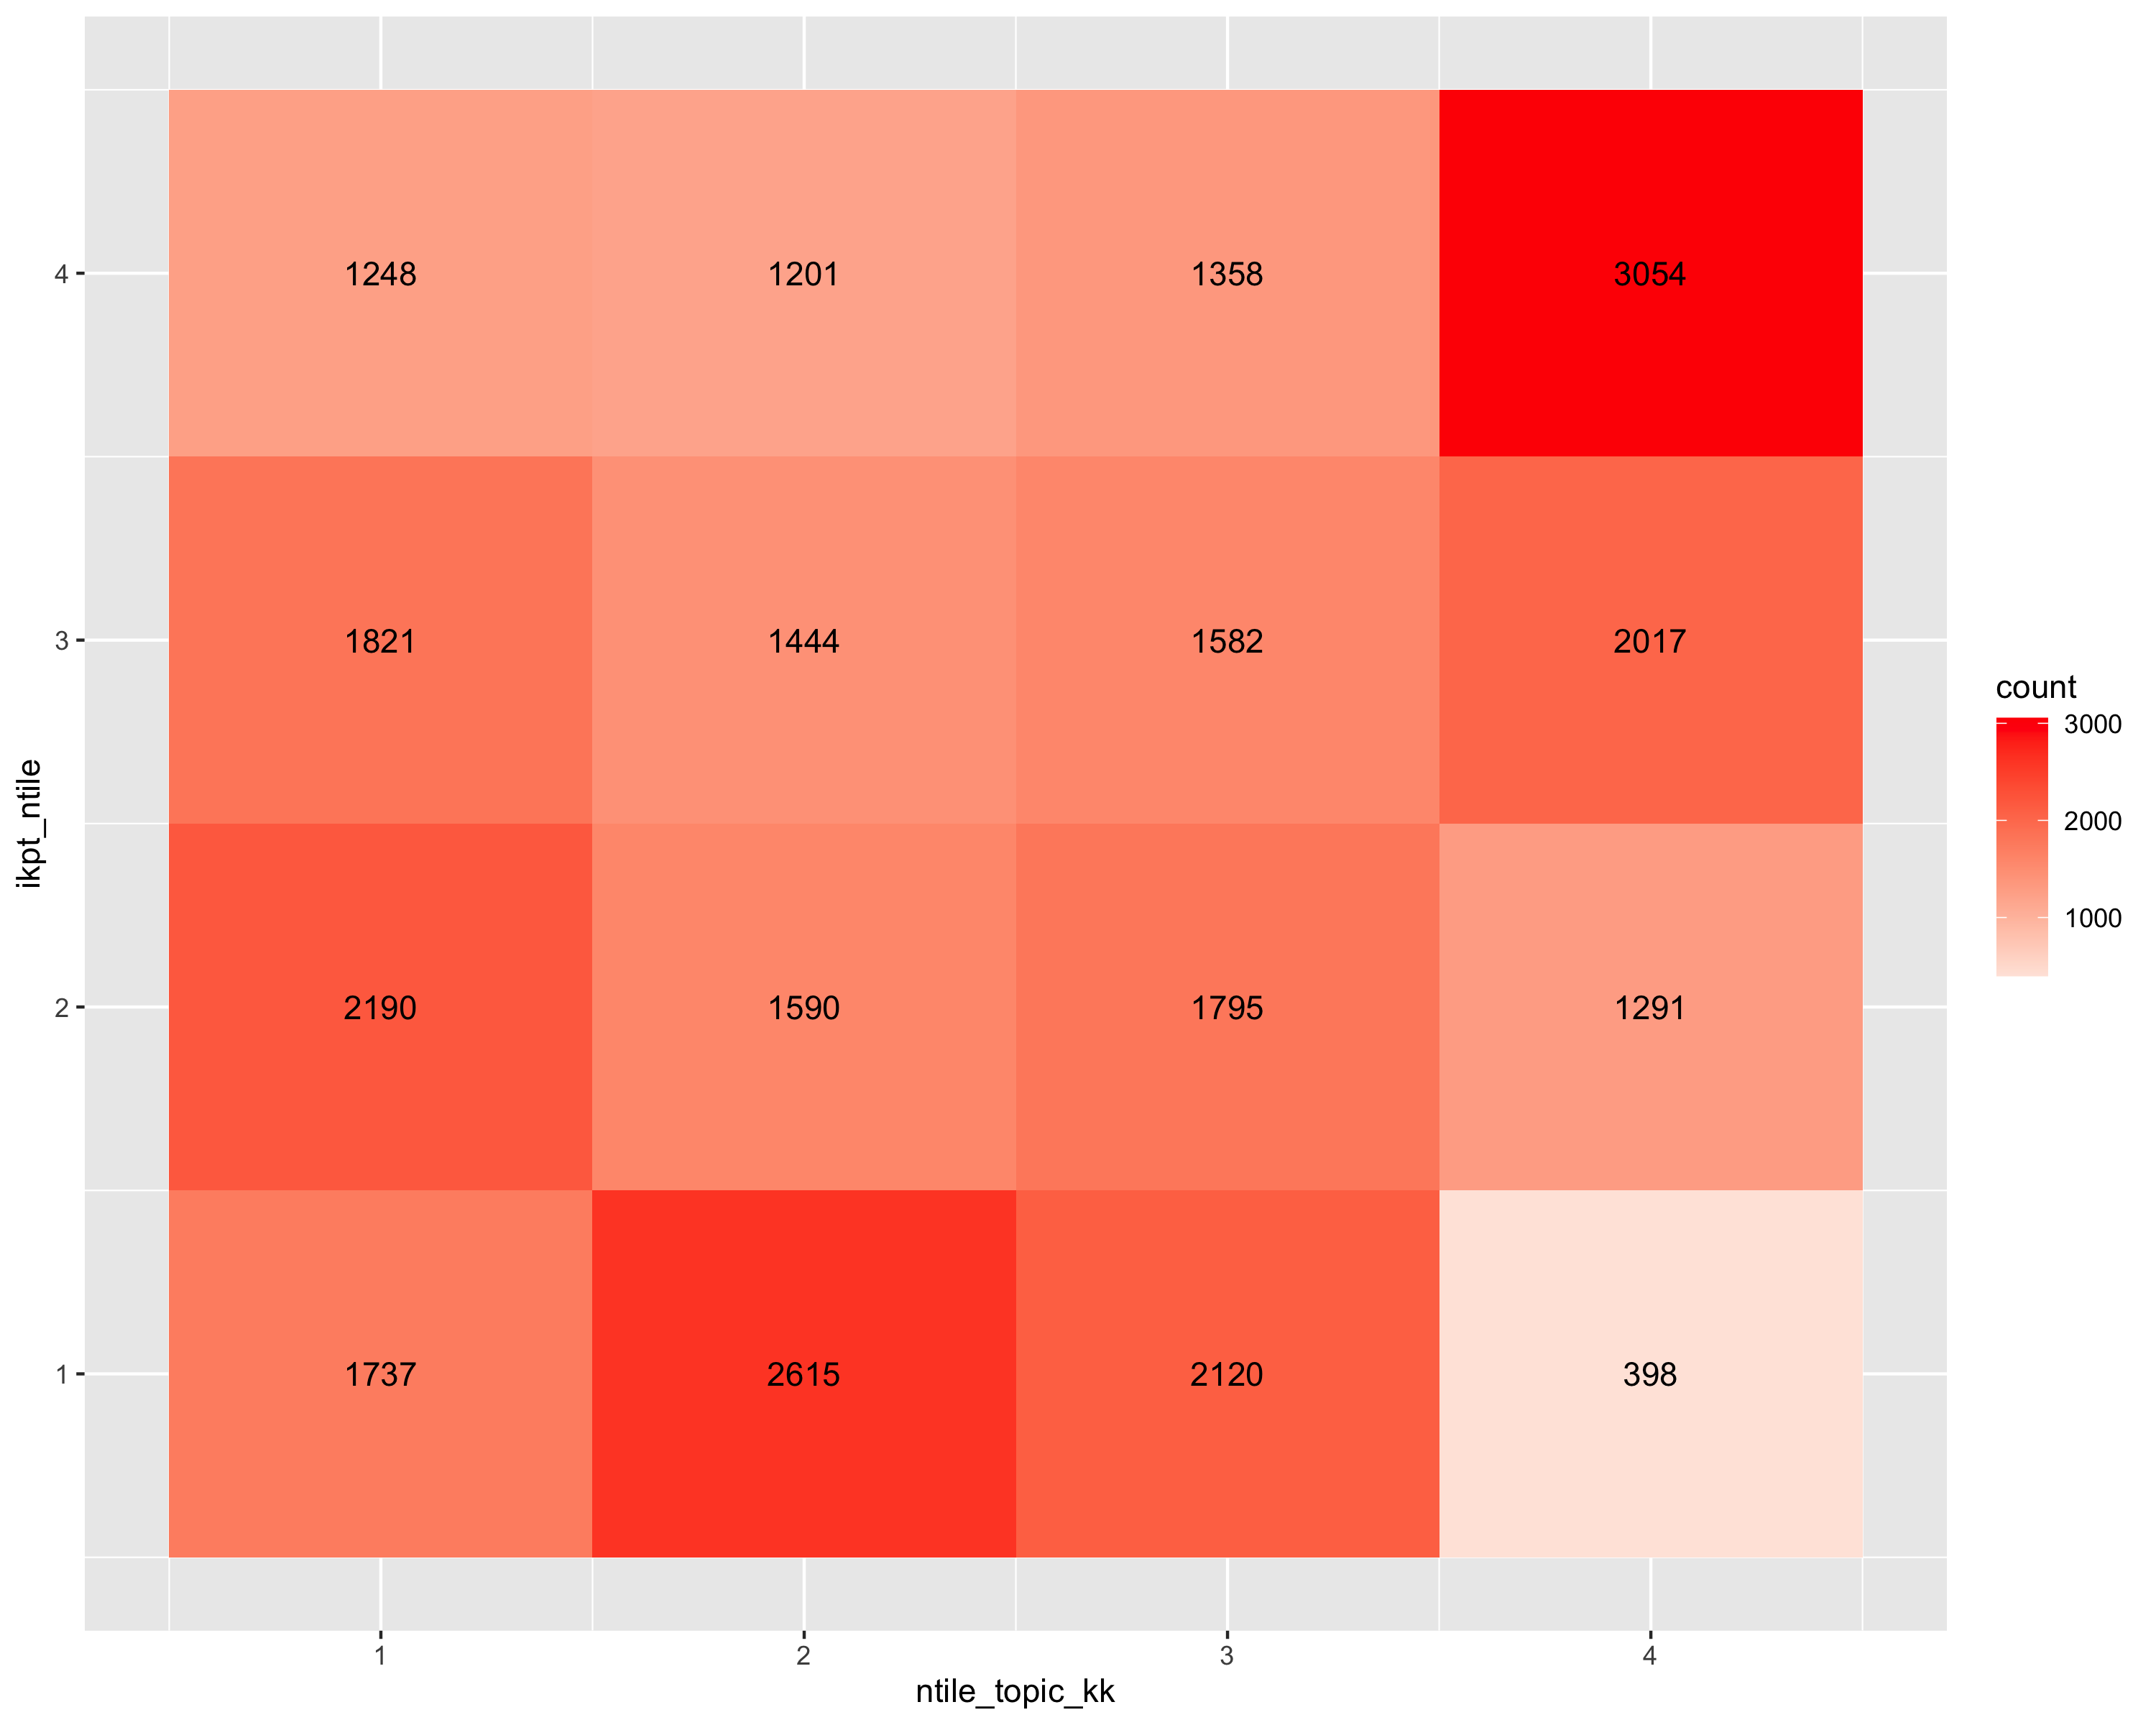
\includegraphics[width=\textwidth]{\ffo/topicvsikpt_hm.png}
		  \centering
		  \captionsetup{font=scriptsize}
		  \label{fig:topicvsikpt_hm}
			\end{figure}
          \column{0.4\linewidth}
          \scriptsize
              \begin{itemize}
			  \item a
			  \item b
			\end{itemize}
	  \end{columns} 
\end{frame}

\begin{frame}
\frametitle{Title}
       \begin{columns}
          \column{0.6\linewidth}
             \begin{figure}[h!]
		  \centering
		  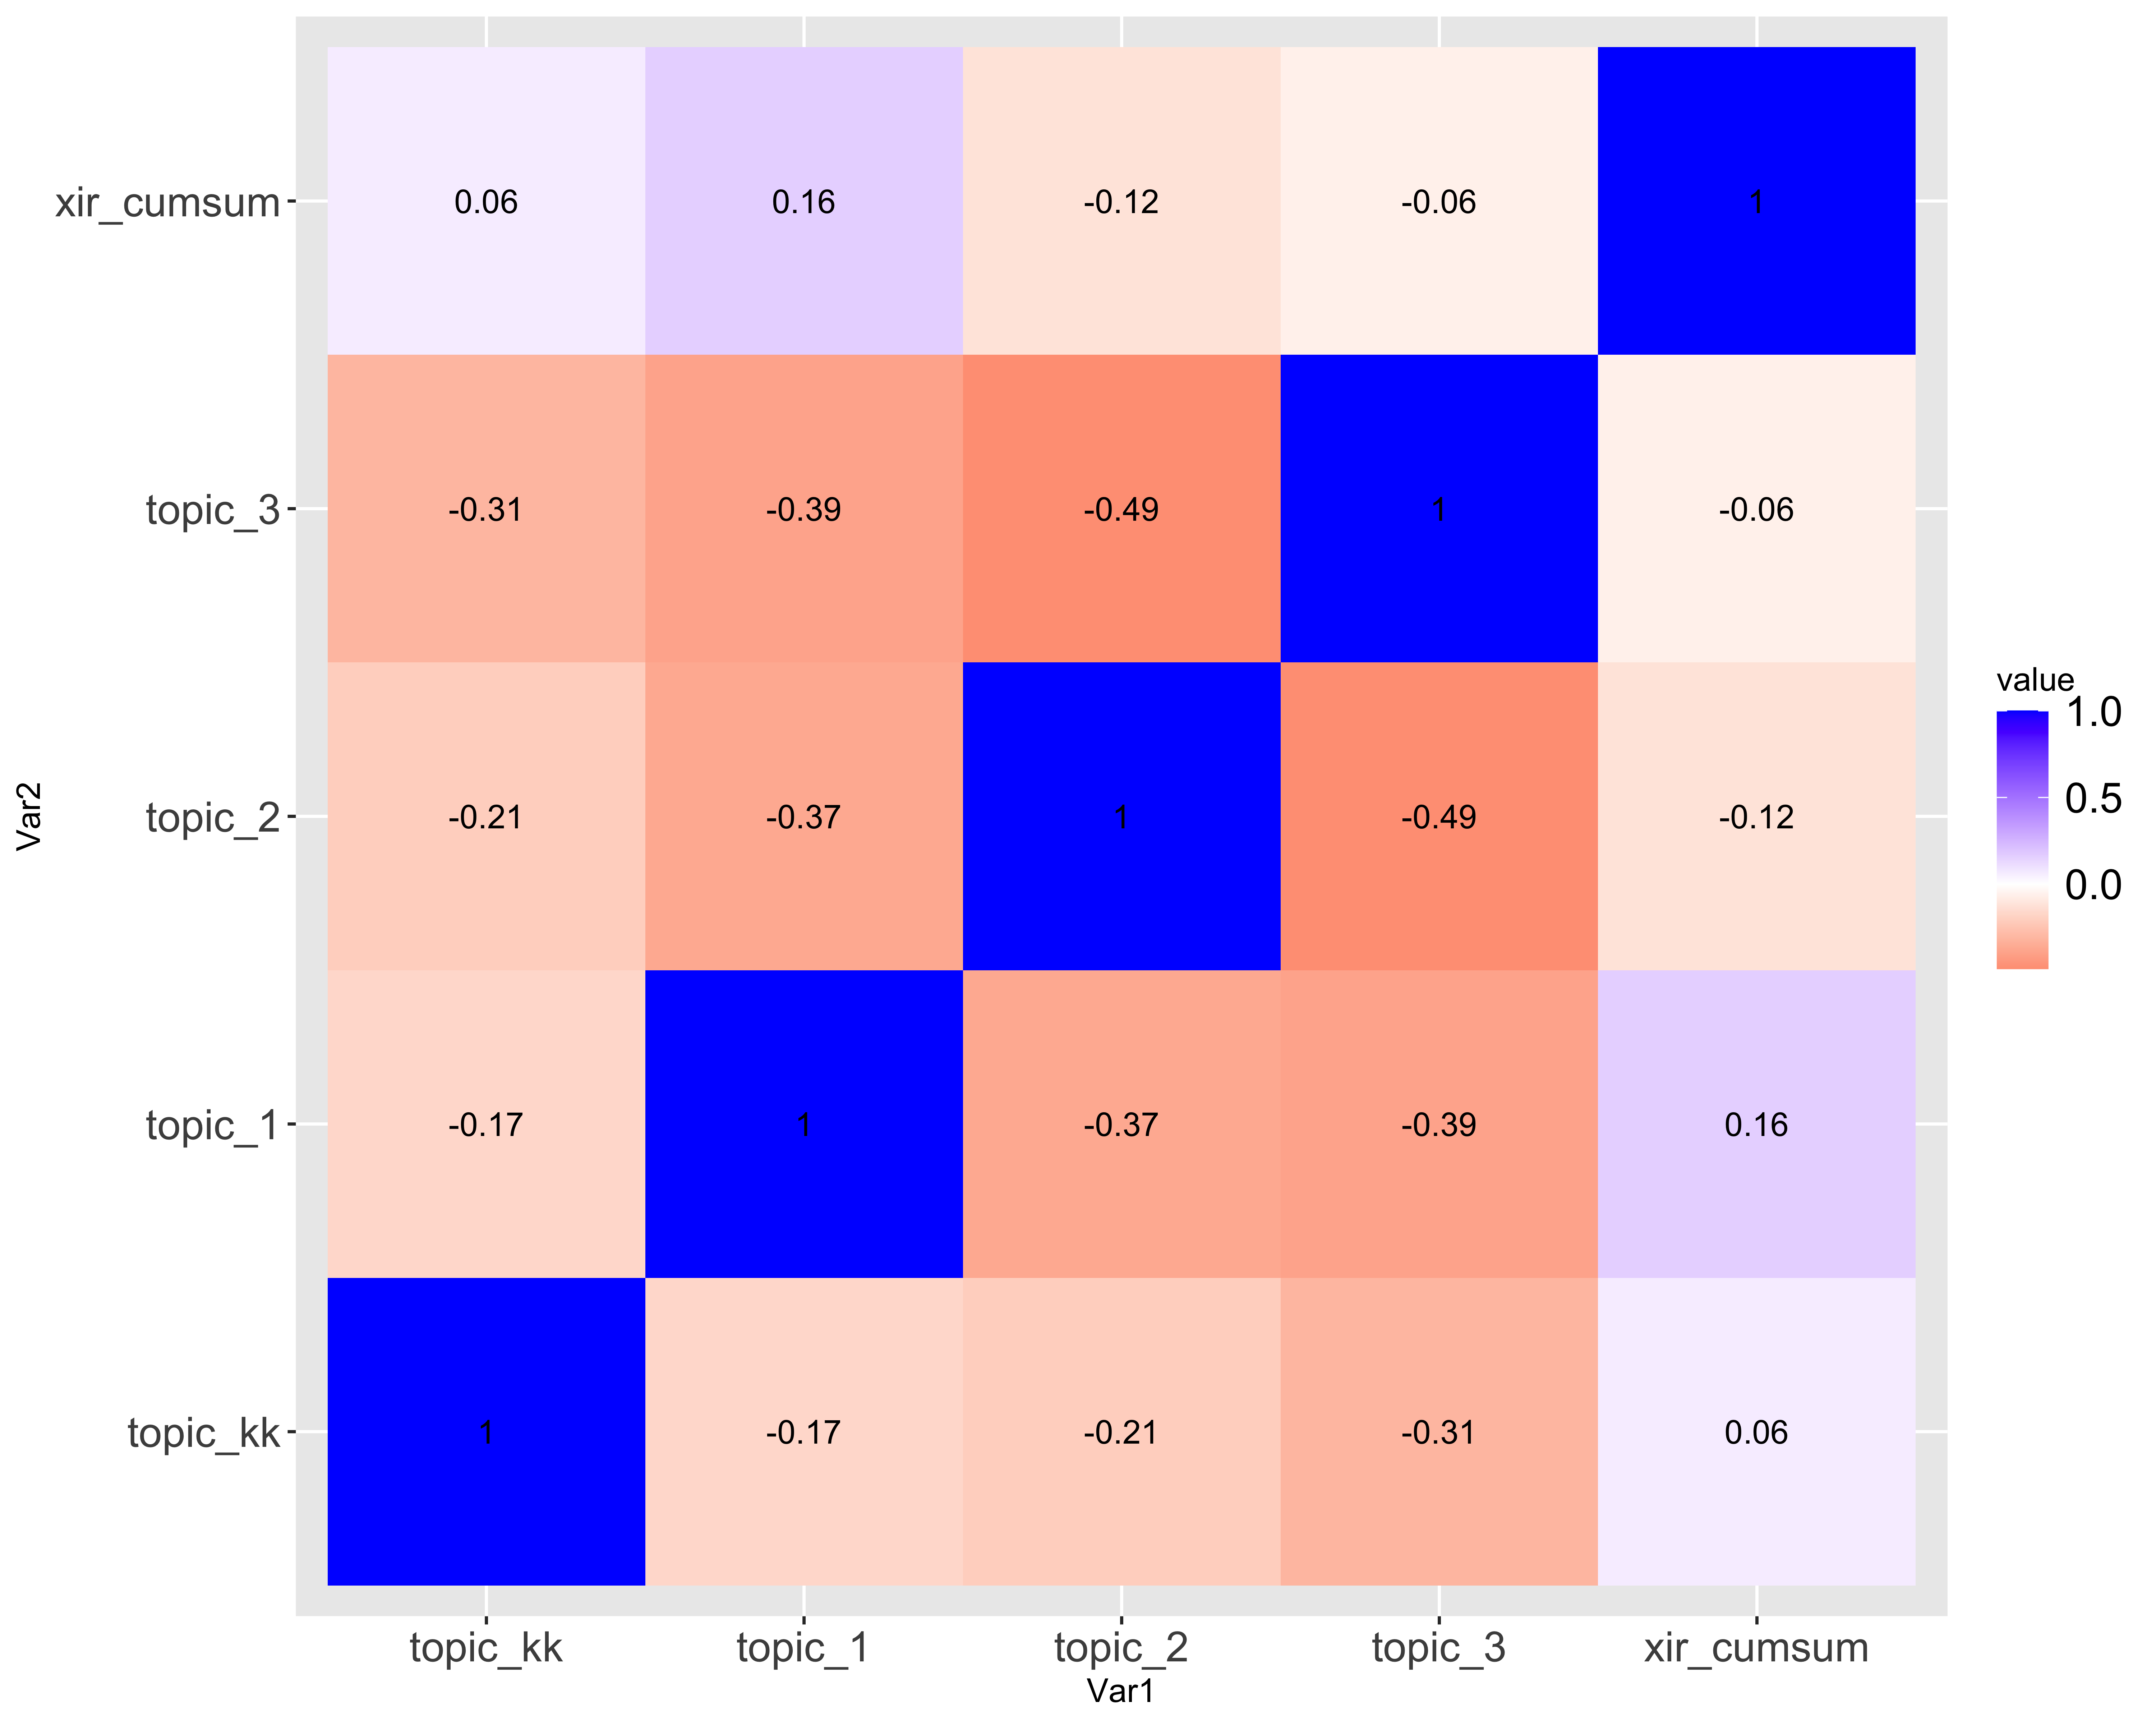
\includegraphics[width=\textwidth]{\ffo/heatmap_patents.png}
		  \captionsetup{font=scriptsize}
		  \label{fig:heatmappatents}
			\end{figure}
          \column{0.4\linewidth}
          \scriptsize
              \begin{itemize}
			  \item a
			  \item b
			\end{itemize}
	  \end{columns} 
\end{frame}

\begin{frame}
\frametitle{Count of firms in the upper quartile of topic\_kk}
\insertfigure{stackedplot_n}{stackedplotn}
\end{frame}

%%%%%%%%%%%%%%%%%%%%%%%%%%%%% ROBUSTNESS TEST: 3 TOPICS
\begin{frame}
\label{robthree}
\centering
\huge\bfseries Robustness tests: 3 topics
\hyperlink{results}{\beamerbutton{Back to results}}
\end{frame}

\begin{frame}
  \frametitle{Defining topic\_kk}
  \begin{itemize}
  \item LDA creates $k$ topics and assigns them to each document of the corpus. "Patents", "intellectual property", and correlated terms tend to be concentrated in few topics.
  \item For every topic map, I define "topic\_kk" as the topic that has the highest loading within high-tech sectors in the economy, defined as SIC codes 283, 357, 466, 367, 382, 384, 737 (\cite{Brown2009-zp}) 
  
\begin{table}[!htbp] \centering 
  \caption{Topic averages by hi-tech status} 
  \label{fig:bytech} 
\begin{tabular}{@{\extracolsep{5pt}} D{.}{.}{-3} D{.}{.}{-3} D{.}{.}{-3} D{.}{.}{-3} D{.}{.}{-3} } 
\\[-1.8ex]\hline 
\hline \\[-1.8ex] 
\multicolumn{1}{c}{hi\_tech} & \multicolumn{1}{c}{topic\_0} & \multicolumn{1}{c}{topic\_1} & \multicolumn{1}{c}{topic\_2} & \multicolumn{1}{c}{topic\_3} \\ 
\hline \\[-1.8ex] 
\multicolumn{1}{c}{0} & \multicolumn{1}{c}{0.018} & \multicolumn{1}{c}{0.459} & \multicolumn{1}{c}{0.267} & \multicolumn{1}{c}{0.253} \\ 
\multicolumn{1}{c}{1} & \multicolumn{1}{c}{0.308} & \multicolumn{1}{c}{0.584} & \multicolumn{1}{c}{0.02} & \multicolumn{1}{c}{0.086} \\ 
\hline \\[-1.8ex] 
\end{tabular} 
\end{table} 

\end{itemize}

\end{frame}


\begin{frame}
\frametitle{Topic\_kk vs. patent activity}
       \begin{columns}
          \column{0.6\linewidth}
             \begin{figure}[h!]
		  \centering
		  \includegraphics[width=\textwidth]{\ffoiii/firmsbypat_hm.png}
		  \captionsetup{font=scriptsize}
		  \label{fig:firmsbypathm}
			\end{figure}
          \column{0.4\linewidth}
          \scriptsize
              \begin{itemize}
              \item Here, I count the co-occurrences of topic\_kk quartiles and accumulated patent-related firm market value.
              \item \cite{Kogan2017-fx} use stock market data to estimate the value of all patents filed by public firms since 1926.
			  \item The vertical axis is divided by yearly defined quartiles of:
			  \begin{equation}
  				\frac{\text{Accumulated Patent Value}}{\text{Total assets}}
				\end{equation}
			  \item A higher accumulated patent value is associated with higher loadings of topic\_kk.
			\end{itemize}
	  \end{columns} 
\end{frame}

\begin{frame}
\frametitle{Topic\_kk vs. Knowledge Capital}
\scriptsize
\insertfigureiii{topicvskkpt_hm}{Correlation between quartiles of Knowledge capital,  as defined in \cite{Peters2017-fl}, vs. quartiles of topic\_kk. Higher accumulated investments in R\&D are correlated to higher loadings of topic\_kk.}
\end{frame}

\begin{frame}
\frametitle{Topic\_kk vs. Skill}
\scriptsize
\insertfigureiii{heatmap}{Correlation between different topics and average industry skill, as measured by \cite{Belo2017-qi}. \cite{Belo2017-qi} define industry skill as defined as the share of high-skill workers measured by the BLS; a "high-skill" occupation has Specific Vocational Preparation $\geq 7$ or over two years of preparation.}. 
\end{frame}

\begin{frame}
\frametitle{Value-weighted returns}

\insertfigureiii{awawr}{Value-weighted accumulated weekly returns; grouped by quartile of topic\_kk (defined every year)}
\end{frame}



\begin{frame}
\frametitle{Value-weighted returns, grouping by topic\_kk (defined for every year-ind12)}
\insertfigureiii{awawr_aggind}{Value-weighted accumulated weekly returns}
\end{frame}

\begin{frame}
\frametitle{Value-weighted returns, defining 4-tiles by year $\times$ ind12}
\insertfigureiii{awawr_byg}{Value-weighted accumulated weekly returns, grouping by firms' maximum topic.}
\end{frame}

\begin{frame}
\frametitle{Different topics are associated with different cross-sectional volatility patterns}
\insertfigureiii{wsdr_byg}{Weekly standard deviation of returns within groups, grouped by maximum topic.}
\end{frame}

\begin{frame}
\frametitle{Accumulated assets of firms in the upper quartile of topic\_kk}
\insertfigureiii{stackedplot_at}{Accumulated assets of firms in the upper quartile of topic\_kk}
\end{frame}


%%%%%%%%%%%%%%%%%%%%%%%%%%%%% ROBUSTNESS TEST: 6 TOPICS
\begin{frame}
\label{robsix}
\centering
\huge\bfseries Robustness tests: 6 topics
\hyperlink{results}{\beamerbutton{Back to results}}
\end{frame}

\begin{frame}
  \frametitle{Defining topic\_kk}
  \begin{itemize}
  \item LDA creates $k$ topics and assigns them to each document of the corpus. "Patents", "intellectual property", and correlated terms tend to be concentrated in few topics.
  \item For every topic map, I define "topic\_kk" as the topic that has the highest loading within high-tech sectors in the economy, defined as SIC codes 283, 357, 466, 367, 382, 384, 737 (\cite{Brown2009-zp}) 
  \tiny
  
\begin{table}[!htbp] \centering 
  \caption{Topic averages by hi-tech status} 
  \label{fig:bytech} 
\begin{tabular}{@{\extracolsep{5pt}} D{.}{.}{-3} D{.}{.}{-3} D{.}{.}{-3} D{.}{.}{-3} D{.}{.}{-3} } 
\\[-1.8ex]\hline 
\hline \\[-1.8ex] 
\multicolumn{1}{c}{hi\_tech} & \multicolumn{1}{c}{topic\_0} & \multicolumn{1}{c}{topic\_1} & \multicolumn{1}{c}{topic\_2} & \multicolumn{1}{c}{topic\_3} \\ 
\hline \\[-1.8ex] 
\multicolumn{1}{c}{0} & \multicolumn{1}{c}{0.018} & \multicolumn{1}{c}{0.459} & \multicolumn{1}{c}{0.267} & \multicolumn{1}{c}{0.253} \\ 
\multicolumn{1}{c}{1} & \multicolumn{1}{c}{0.308} & \multicolumn{1}{c}{0.584} & \multicolumn{1}{c}{0.02} & \multicolumn{1}{c}{0.086} \\ 
\hline \\[-1.8ex] 
\end{tabular} 
\end{table} 

\end{itemize}

\end{frame}


\begin{frame}
\frametitle{Topic\_kk vs. patent activity}
       \begin{columns}
          \column{0.6\linewidth}
             \begin{figure}[h!]
		  \centering
		  \includegraphics[width=\textwidth]{\ffovi/firmsbypat_hm.png}
		  \captionsetup{font=scriptsize}
		  \label{fig:firmsbypathm}
			\end{figure}
          \column{0.4\linewidth}
          \scriptsize
              \begin{itemize}
              \item Here, I count the co-occurrences of topic\_kk quartiles and accumulated patent-related firm market value.
              \item \cite{Kogan2017-fx} use stock market data to estimate the value of all patents filed by public firms since 1926.
			  \item The vertical axis is divided by yearly defined quartiles of:
			  \begin{equation}
  				\frac{\text{Accumulated Patent Value}}{\text{Total assets}}
				\end{equation}
			  \item A higher accumulated patent value is associated with higher loadings of topic\_kk.
			\end{itemize}
	  \end{columns} 
\end{frame}

\begin{frame}
\frametitle{Topic\_kk vs. Knowledge Capital}
\scriptsize
\insertfigurevi{topicvskkpt_hm}{Correlation between quartiles of Knowledge capital,  as defined in \cite{Peters2017-fl}, vs. quartiles of topic\_kk. Higher accumulated investments in R\&D are correlated to higher loadings of topic\_kk.}
\end{frame}

\begin{frame}
\frametitle{Topic\_kk vs. Skill}
\scriptsize
\insertfigurevi{heatmap}{Correlation between different topics and average industry skill, as measured by \cite{Belo2017-qi}. \cite{Belo2017-qi} define industry skill as defined as the share of high-skill workers measured by the BLS; a "high-skill" occupation has Specific Vocational Preparation $\geq 7$ or over two years of preparation.}. 
\end{frame}

\begin{frame}
\frametitle{Value-weighted returns}
\insertfigurevi{awawr}{Value-weighted accumulated weekly returns; grouped by quartile of topic\_kk (defined every year)}
\end{frame}



\begin{frame}
\frametitle{Value-weighted returns, grouping by topic\_kk (defined for every year-ind12)}
\insertfigurevi{awawr_aggind}{Value-weighted accumulated weekly returns}
\end{frame}

\begin{frame}
\frametitle{Value-weighted returns, defining 4-tiles by year $\times$ ind12}
\insertfigurevi{awawr_byg}{Value-weighted accumulated weekly returns, grouping by firms' maximum topic.}
\end{frame}

\begin{frame}
\frametitle{Different topics are associated with different cross-sectional volatility patterns}
\insertfigurevi{wsdr_byg}{Weekly standard deviation of returns within groups, grouped by maximum topic.}
\end{frame}

\begin{frame}
\frametitle{Accumulated assets of firms in the upper quartile of topic\_kk}
\insertfigurevi{stackedplot_at}{Accumulated assets of firms in the upper quartile of topic\_kk}
\end{frame}


\end{document}
